% VisTacFusion Architecture Diagram
% Compile with: pdflatex -shell-escape architecture_diagram.tex
% Requires: tikz, graphicx
% Place image assets in same directory or adjust paths

\documentclass[border=10pt]{standalone}
\usepackage{tikz}
\usepackage{graphicx}
\usepackage{amsmath}
\usepackage{amssymb}

\usetikzlibrary{
  arrows.meta,
  positioning,
  fit,
  backgrounds,
  calc,
  decorations.pathreplacing,
  shapes.geometric
}

\definecolor{encoderblue}{HTML}{D6EAF8}
\definecolor{encoderborder}{HTML}{5DADE2}
\definecolor{projgray}{HTML}{E8E8E8}
\definecolor{projborder}{HTML}{AAAAAA}
\definecolor{trunkgreen}{HTML}{D5F5E3}
\definecolor{trunkborder}{HTML}{58D68D}
\definecolor{dptpath}{HTML}{FFF3CD}
\definecolor{dptborder}{HTML}{F0C040}
\definecolor{headpurple}{HTML}{E8DAEF}
\definecolor{headborder}{HTML}{AF7AC5}
\definecolor{inputtac}{HTML}{FDEBD0}
\definecolor{inputrgb}{HTML}{D4E6F1}
\definecolor{bottleneck}{HTML}{D1F2EB}
\definecolor{bnborder}{HTML}{1ABC9C}
\definecolor{outputdepth}{HTML}{F2F3F4}
\definecolor{outputborder}{HTML}{95A5A6}
\definecolor{tapinject}{HTML}{FDEBD0}
\definecolor{tapborder}{HTML}{E59866}

\tikzset{
  block/.style={
    draw, rounded corners=3pt, minimum height=1.0cm,
    minimum width=2.0cm, align=center, font=\footnotesize,
    inner sep=4pt, line width=0.6pt,
  },
  encoder/.style={block, fill=encoderblue, draw=encoderborder, minimum width=2.8cm, minimum height=1.2cm},
  proj/.style={block, fill=projgray, draw=projborder, minimum width=1.8cm, minimum height=0.8cm},
  trunk/.style={block, fill=trunkgreen, draw=trunkborder, minimum width=3.0cm, minimum height=2.2cm},
  head/.style={block, fill=headpurple, draw=headborder, minimum width=1.8cm, minimum height=0.9cm},
  dptblock/.style={block, fill=dptpath, draw=dptborder, minimum width=2.2cm},
  tapblock/.style={block, fill=tapinject, draw=tapborder, minimum width=2.2cm},
  output/.style={block, fill=outputdepth, draw=outputborder, minimum width=1.6cm, minimum height=0.8cm},
  bnblock/.style={block, fill=bottleneck, draw=bnborder, minimum width=2.0cm, minimum height=0.8cm},
  imgnode/.style={inner sep=0pt, outer sep=0pt},
  arr/.style={-{Stealth[length=5pt, width=4pt]}, line width=0.7pt, color=#1},
  arr/.default={black!70},
  darr/.style={-{Stealth[length=5pt, width=4pt]}, line width=0.7pt, dashed, color=#1},
  darr/.default={black!50},
  lblsmall/.style={font=\scriptsize, text=black!60},
  lbltiny/.style={font=\tiny, text=black!50},
  pathbox/.style={draw=#1, rounded corners=5pt, line width=1.0pt, dashed, inner sep=8pt},
}

\begin{document}
\begin{tikzpicture}[node distance=0.6cm and 0.8cm]

% ============================================================
% INPUT IMAGES (left side)
% ============================================================

% Tactile input
\node[imgnode] (tac_img) {%
  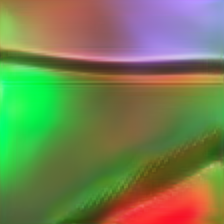
\includegraphics[width=1.4cm]{assets/tactile_sim.png}%
};
\node[below=0.05cm of tac_img, font=\scriptsize\bfseries, text=black!70] {Tactile};

% RGB input (below tactile)
\node[imgnode, below=2.0cm of tac_img] (rgb_img) {%
  
\includegraphics[width=1.4cm]{assets/rgb_sim.png}%
};
\node[below=0.05cm of rgb_img, font=\scriptsize\bfseries, text=black!70] {RGB};

% ============================================================
% ENCODERS
% ============================================================

% Tactile encoder
\node[encoder, right=1.2cm of tac_img] (tac_enc) {
  \textbf{Tactile Encoder}\\[-1pt]
  {\tiny (T3 ViT-L/16, \textit{frozen})}
};

% RGB encoder
\node[encoder, right=1.2cm of rgb_img] (rgb_enc) {
  \textbf{RGB Encoder}\\[-1pt]
  {\tiny (MAE ViT-L/16, \textit{frozen})}
};

% Arrows: input -> encoder
\draw[arr] (tac_img) -- (tac_enc);
\draw[arr] (rgb_img) -- (rgb_enc);

% ============================================================
% DPT PATH (top)
% ============================================================

% Multiscale taps
\node[dptblock, above right=0.8cm and 1.0cm of tac_enc, minimum height=0.9cm] (ms_taps) {
  \textbf{Multiscale Taps}\\[-2pt]
  {\tiny $4 \times [B, 196, 1024]$}
};

% TapInjection
\node[tapblock, right=0.8cm of ms_taps, minimum height=0.9cm] (tap_inject) {
  \textbf{TapInjection}\\[-2pt]
  {\tiny $\mathbf{t}' = \mathbf{t} + \alpha \cdot \mathrm{CA}(\mathbf{t}, \mathbf{b})$}\\[-2pt]
  {\tiny $\alpha_{\mathrm{init}} = 0$}
};

% DPT Decoder
\node[head, right=0.8cm of tap_inject, minimum width=2.0cm] (dpt_dec) {
  \textbf{DPT}\\
  \textbf{Decoder}
};

% Output images
\node[imgnode, right=0.8cm of dpt_dec, yshift=0.5cm] (depth_out) {%
  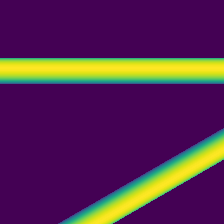
\includegraphics[width=1.1cm]{assets/depth_gt.png}%
};
\node[right=0.02cm of depth_out, font=\scriptsize\bfseries, text=black!70] {Depth};

\node[imgnode, right=0.8cm of dpt_dec, yshift=-0.5cm] (normal_out) {%
  
\includegraphics[width=1.1cm]{assets/normal_gt.png}%
};
\node[right=0.02cm of normal_out, font=\scriptsize\bfseries, text=black!70] {Normal};

% DPT path arrows
\draw[arr] (ms_taps) -- (tap_inject);
\draw[arr] (tap_inject) -- (dpt_dec);
\draw[arr] (dpt_dec) -- (depth_out);
\draw[arr] (dpt_dec) -- (normal_out);

% Encoder -> multiscale taps
\draw[arr] (tac_enc.north) |- (ms_taps.west)
  node[pos=0.25, above, lblsmall] {$4 \times [196, 1024]$};

% ============================================================
% POSE PATH (middle-bottom)
% ============================================================

% Tactile projection
\node[proj, right=1.0cm of tac_enc, yshift=-0.3cm] (tac_proj) {
  \textbf{Proj}\\[-2pt]
  {\tiny $1024 \to 768$}
};

% RGB projection
\node[proj, right=1.0cm of rgb_enc] (rgb_proj) {
  \textbf{Proj}\\[-2pt]
  {\tiny $1024 \to 768$}
};

% Queries
\node[proj, right=0.6cm of tac_proj, minimum width=1.6cm] (queries) {
  \textbf{Queries}\\[-2pt]
  {\tiny $197 \times 768$}
};

% Memory
\node[proj, right=0.6cm of rgb_proj, minimum width=1.6cm] (memory) {
  \textbf{Memory}\\[-2pt]
  {\tiny $197 \times 768$}
};

% Encoder -> projections
\draw[arr] (tac_enc.east) -- (tac_proj.west)
  node[midway, above, lbltiny] {patch+CLS};
\draw[arr] (rgb_enc.east) -- (rgb_proj.west)
  node[midway, above, lbltiny] {patch+CLS};

% Proj -> Queries/Memory
\draw[arr] (tac_proj) -- (queries) node[midway, above, lbltiny] {+pos};
\draw[arr] (rgb_proj) -- (memory);

% ============================================================
% FUSION TRUNK
% ============================================================

\node[trunk, right=0.8cm of $(queries.east)!0.5!(memory.east)$] (trunk) {
  \textbf{Fusion Trunk} $\times 4$\\[4pt]
  {\scriptsize \ding{192} BN $\leftarrow$ Memory}\\[-1pt]
  {\scriptsize \ding{193} Queries $\leftarrow$ BN}\\[-1pt]
  {\scriptsize \ding{194} Queries self-attn}
};

% Bottleneck label inside trunk
\node[bnblock, anchor=north] at ($(trunk.north)-(0, 0.2)$) (bn) {
  \textbf{Bottleneck}\\[-2pt]
  {\tiny $m{=}16, 768$}
};

% Queries -> Trunk
\draw[arr] (queries.east) -- (trunk.west |- queries)
  node[midway, above, lbltiny] {};
% Memory -> Trunk
\draw[arr] (memory.east) -- (trunk.west |- memory);

% ============================================================
% POSE HEAD
% ============================================================

% Pose token
\node[proj, right=0.8cm of trunk, yshift=0.0cm, minimum width=1.4cm] (pose_tok) {
  \textbf{Pose}\\[-2pt]
  \textbf{token}
};

% Pose MLP
\node[head, right=0.6cm of pose_tok, minimum width=1.6cm] (pose_mlp) {
  \textbf{Pose}\\
  \textbf{MLP}
};

% SE(2) output
\node[output, right=0.6cm of pose_mlp, minimum width=2.2cm] (se2) {
  \textbf{SE(2)}\\[-2pt]
  {\tiny $\cos\theta, \sin\theta, t_x, t_y$}
};

% Trunk -> Pose token -> Pose MLP -> SE(2)
\draw[arr] (trunk.east |- pose_tok) -- (pose_tok);
\draw[arr] (pose_tok) -- (pose_mlp)
  node[midway, below, lbltiny] {+spatial pool};
\draw[arr] (pose_mlp) -- (se2);

% ============================================================
% BOTTLENECK -> TAP INJECTION (cross-path connection)
% ============================================================

\draw[darr={black!50}] (bn.north) |- (tap_inject.south)
  node[pos=0.75, right, lbltiny] {bottleneck};

% ============================================================
% DPT PATH BOX
% ============================================================

\begin{scope}[on background layer]
  \node[pathbox=dptborder, fill=dptpath!20,
    fit=(ms_taps)(tap_inject)(dpt_dec),
    label={[font=\footnotesize\bfseries, text=dptborder!80!black]above:DPT Path}
  ] (dptbox) {};
\end{scope}

% ============================================================
% POSE PATH BOX
% ============================================================

\begin{scope}[on background layer]
  \node[pathbox=trunkborder, fill=trunkgreen!15,
    fit=(tac_proj)(rgb_proj)(queries)(memory)(trunk)(pose_tok)(pose_mlp)(se2),
    label={[font=\footnotesize\bfseries, text=trunkborder!80!black]below:Pose Path}
  ] (posebox) {};
\end{scope}

% ============================================================
% MODALITY DROPOUT ANNOTATION
% ============================================================

\node[below=0.3cm of posebox, font=\scriptsize, text=black!60] {
  Modality dropout: $p_{\mathrm{both}}{=}0.55$, \
  $p_{\mathrm{tac}}{=}0.35$, \
  $p_{\mathrm{rgb}}{=}0.10$
};

\end{tikzpicture}
\end{document}
